%% Master Thesis Table of Contents
%% Integrating Object-Centric Learning with Model-Based Reinforcement Learning

\documentclass[
	english,
	ruledheaders=section,
	class=report,
	thesis={type=master},
	accentcolor=9c,
	custommargins=true,
	marginpar=false,
	parskip=half-,
	fontsize=11pt,
]{tudapub}



\usepackage{iftex}
\ifPDFTeX
	\usepackage[utf8]{inputenc}
\fi



%%%%%%%%%%%%%%%%%%%
% Language settings
%%%%%%%%%%%%%%%%%%%
\usepackage{babel}
\usepackage[autostyle]{csquotes}
\usepackage{microtype}


%%%%%%%%%%%%%%%%%%%
% Bibliography
%%%%%%%%%%%%%%%%%%%
\usepackage{biblatex}
\addbibresource{references.bib}


\DefineBibliographyStrings{english}{
  bibliography = {References},
}


%%%%%%%%%%%%%%%%%%%
% Table packages
%%%%%%%%%%%%%%%%%%%
\usepackage{tabularx}
\usepackage{booktabs}

%%%%%%%%%%%%%%%%%%%
% Math packages
%%%%%%%%%%%%%%%%%%%
\usepackage{mathtools}
\usepackage{amssymb}
\usepackage{siunitx}

%%%%%%%%%%%%%%%%%%%
% Additional packages
%%%%%%%%%%%%%%%%%%%
\usepackage{algorithm}
\usepackage{algorithmic}
\usepackage{listings}
\usepackage{xcolor}
\usepackage{graphicx}
\usepackage{subcaption}

\begin{document}

\Metadata{
	title=Structured World Understanding: Integrating Object-Centric Learning with Model-Based Reinforcement Learning,
	author=Your Name
}

\title{Structured World Understanding: Integrating Object-Centric Learning with Model-Based Reinforcement Learning}
\subtitle{Master's Thesis: Summer Semester 2025}
\author[Y. Name]{Your Full Name}
\studentID{1234567}
\reviewer{Jannis Blüml}

\department{Department of Computer Science}
\institute{Institute of Computer Science}
\group{Machine Learning Research Group}

\submissiondate{24.10.2025}
\examdate{24.10.2025}

\maketitle

\affidavit

\tableofcontents
\listoffigures
\listoftables

% List of Abbreviations
\chapter*{List of Abbreviations}
\addcontentsline{toc}{chapter}{List of Abbreviations}
\begin{tabular}{ll}
	RL   & Reinforcement Learning              \\
	MBRL & Model-Based Reinforcement Learning  \\
	MFRL & Model-Free Reinforcement Learning   \\
	CNN  & Convolutional Neural Network        \\
	LSTM & Long Short-Term Memory              \\
	PPO  & Proximal Policy Optimization        \\
	A3C  & Asynchronous Advantage Actor-Critic \\
	DQN  & Deep Q-Network                      \\
	RSSM & Recurrent State Space Model         \\
	KL   & Kullback-Leibler                    \\
	MSE  & Mean Squared Error                  \\
	RGB  & Red-Green-Blue                      \\
	GPU  & Graphics Processing Unit            \\
	JAX  & Just After eXecution                \\
\end{tabular}

\chapter{Introduction}
\label{chap:introduction}

Reinforcement Learning as one of the three flavors in Machine Learning among
Supervised and Unsupervised Learning follows the approach of having an agent
performs actions in an environment and receiving rewards for certain actions.
So unlike Supervised Learning for example there is no ground truth from the
which the agent can learn from. Among numerous distinctions within
Reinforcement Learning there is the difference between Model Based
Reinforcement Learning and Model Free Reinforcement Learning. The latter
focuses on the learning of only the Agent which is deployed in the environment
(or learns from samples). Thus the agent will have no explicit way of
predicting the next state of the environment, although sufficiently large for
example neural networks might create some implicit model of the world. Model
based Reinforcement learning augments the architecture by a Model that is
predicting the next state of the world but also still trains an agent. Although
model free approaches usually are less complex since they only have to learn
one model, the agent they also have significant disadvantages.

Model Free Learning approaches often struggle with sample efficiency and
generalization to new tasks. Small changes in the environment can lead to
significant drops in performance. Moreover, agents can learn misaligned
policies that exploit loopholes in the environment rather than achieving the
intended goals. These challenges highlight the need for more structured and
interpretable learning methods. So Object Centricity and Model Based approaches
both have the goal of improving abstract reasoning by developing a more
abstract understanding of the world and improving sample efficiency. This
thesis aims to investigate the potential benefits of integrating object-centric
learning into model-based reinforcement learning frameworks to address these
challenges by harvesting the strengths of both paradigms. This thesis is
therefore guided by the following research questions:
\begin{enumerate}
	\item How do object-centric world models compare to pixel-based world models
	      regarding prediction accuracy and sample efficiency?
	\item Can an actor-critic framework be effectively trained on simulated rollouts from
	      object-centric world models?
	\item What is the impact of different world model architectures (such as LSTM-based
	      versus alternative designs) on the overall performance of object-centric
	      model-based reinforcement learning in structured environments?
	\item Does the object-centric inductive bias in world models improve robustness to
	      changes in the environment?
\end{enumerate}

Within this thesis we propose to develop a world model that is running on top
of object centric states provided by the JAXAtari framework. This world model
will be based on an LSTM architecture and will be trained to predict the next
state of the environment given the current state and action. An actor-critic
framework based on the DreamerV2 architecture will be integrated with the world
model to learn policies from imagined rollouts. The training pipeline will
involve alternating between updating the world model and optimizing the policy
based on simulated experiences. The performance of the proposed approach will
be evaluated in the Pong environment from the Atari benchmark suite, comparing
it against pixel-based baselines and assessing its sample efficiency and
robustness.

The remainder of this thesis is structured as follows: Chapter 2 provides
background information on reinforcement learning, model-based approaches, and
object-centric representations. Chapter 3 details the methodology, including
the world model architecture, actor-critic integration, and training pipeline.
Chapter 4 presents the experimental setup, results, and analysis. Chapter 5
discusses the findings, challenges, and implications of the results. Finally,
Chapter 6 concludes the thesis and outlines directions for future work.

\chapter{Background and Related Work}
\label{chap:background}
This chapter aims to give an overview into the relevant mathematical background and related work
in the fields of Reinforcement Learning, Model-Based Reinforcement Learning and Object-Centric Learning.
\section{Reinforcement Learning}
\label{sec:reinforcement_learning}

Reinforcement Learning (RL) is a machine learning subcategory that focuses on
training agents that make decision in an environment. An environment can be a
game, a robotic control task or any other sequential decision making problem.
To give that a more structured formulation the definition of a Markov Decision
Process (MDP) is used. This term comes from the field of operations research
and was named after the Russian mathematician Andrey Markov in relation to his
work on stochastic processes. An MDP is defined as a tuple $\mathcal{M} =
	(\mathcal{S}, \mathcal{A}, P, R, \gamma)$, where:

\begin{itemize}
	\item $\mathcal{S}$ is the state space
	\item $\mathcal{A}$ is the action space
	\item $P(s'|s,a)$ is the transition probability function defining the probability of transitioning to state $s'$ given current state $s$ and action $a$
	\item $R(s,a,s')$ is the reward function specifying the immediate reward received after taking action $a$ in state $s$ and transitioning to state $s'$
	\item $\gamma \in [0,1]$ is the discount factor that determines the importance of future rewards. This is also often used to prove convergence of certain algorithms.
\end{itemize}

Markov Chains assume the Markov property, which states that the future state
depends only on the current state and action, not on the entire history of past
states and actions. This memoryless property is what enabled many
computationally viable algorithms to be developed in the first place since
every probability computed is only conditioned on the current state and action
so a finite set of values instead of a potentially infinite set of past states
and actions.

Given that we now defined what the environment actually means let us examine at the
goal of the agent. The agent's goal is to learn an optimal policy $\pi^*(s)$
that maximizes the expected cumulative discounted reward, known as the return:
\begin{equation}
	G_t = \sum_{k=0}^{\infty} \gamma^k R_{t+k+1}
\end{equation}

The value function $V^\pi(s)$ represents the expected return when starting from
state $s$ and following policy $\pi$:
\begin{equation}
	V^\pi(s) = \mathbb{E}_\pi[G_t | S_t = s]
\end{equation}

In a similar manner, $Q^\pi(s,a)$ represents the expected return when starting
from state $s$, taking action $a$, and then following policy $\pi$. Making the
action value function a function of both state and action. This can sometimes
be more useful since it directly tells you the value of taking a certain action
as well.

Model-free reinforcement learning approaches learn optimal policies directly
from experience without explicitly modeling the environment dynamics. These
methods estimate value functions or policies through trial-and-error
interactions with the environment, making them broadly applicable but
potentially sample-inefficient.

As mentioned in the introduction, model-free rely on learning an agent directly
by interacting with the environment and receiving feedback in the form of
rewards. This trial-and-error process allows the agent to improve its policy
over time. By omitting a world model the complexity of the overall system is
reduced but the the agent is usually quite sample inefficient
\cite{mnih2015human}. Also, the lack of a model can make it difficult for the
agent to plan ahead or consider the long-term consequences of its actions. On
top of that world models can improve generalization to new tasks and make the
agent more robust \cite{ha2018world}. Moreover they provide limited
interpretability with regards to their learned policy.

Popular model-free algorithms include temporal difference methods like
Q-Learning and SARSA, as well as policy gradient methods such as REINFORCE,
Actor-Critic, and Proximal Policy Optimization (PPO).

Model-based reinforcement learning addresses some limitations of model-free
approaches by learning an explicit model of the environment dynamics.

The world model typically learns to predict next states and rewards given
current states and actions:

\begin{align}
	\hat{s}_{t+1} & = f_\theta(s_t, a_t)        \\
	\hat{r}_{t+1} & = g_\phi(s_t, a_t, s_{t+1})
\end{align}

where $f_\theta$ and $g_\phi$ represent parameterized functions (often neural
networks) that approximate the true environment dynamics. Sometimes the reward
prediction can be omitted if the reward can somehow be directly read out from
the game itself which is common in Atari games for example assuming there
exists an object centric approach that encompasses the score.

Model-based methods potentially have much better sample efficiency since it
takes less sampling in the environment to learn reasonable state transitions
than it takes to train a reinforcement learning. After the Model has been
properly trained the agent can learn entirely within the worldmodel making
additional sampling unnecessary. Although depending on game complexity the
initial sampling which is usually done by a random policy might not see diverse
enough states. This is for most Atari Games not an Issue but for more complex
environments it can be important to retrain the worldmodel with new experience
that is sampled by the now trained (within the model) trained agent in the real
environment \cite{hafner2019dreamer}. Moreover there are approaches that use
explicit planning strategies that hugely benefit interpretability. Using the
worldmodel the Agent can make guesses what might happen in the future and
explicitly reason why it decides for a certain action
\cite{schrittwieser2020mastering}.

But training a well designed and stable model can create several challenges for
example the world model can introduce a bias into the agent which doesnt hold
in the true environment. The agent can learn to exploit errors in the
worldmodel to artificially boost its score but then performing much worse
during inference \cite{lambert2020objective}.

\section{Dreamer Architecture}
\label{sec:dreamer_architecture}

The Dreamer architecture is a family of model-based RL algorithms (DreamerV1,
V2, V3) that use a world model together with actor-critic methods. The main
idea is to learn a compact latent space where the agent can imagine rollouts
and train its policy without always interacting with the real environment.
Dreamer builds on ideas from PlaNet, which first used latent dynamics, but
Dreamer adds actor-critic learning and works better for Atari games.

DreamerV2 improves DreamerV1 by making it more stable and able to handle
discrete actions, which is important for Atari. DreamerV3 tries to make the
method work for many different tasks without changing hyperparameters. There
are different ways to train a world model. You can predict future observations
directly or predict latent states. Also, there are many possible architectures
for the world model, like MLPs, LSTMs, or Transformers.DreamerV2
\cite{hafner2019dreamer} is a model-based RL algorithm. In general, Dreamer
works by learning a world model, then using it to imagine future states, and
then training the actor and critic on these imagined rollouts. The world model
predicts what will happen next, the actor tries to choose good actions, and the
critic estimates how good a state is.

\begin{figure}[ht]
	\centering
	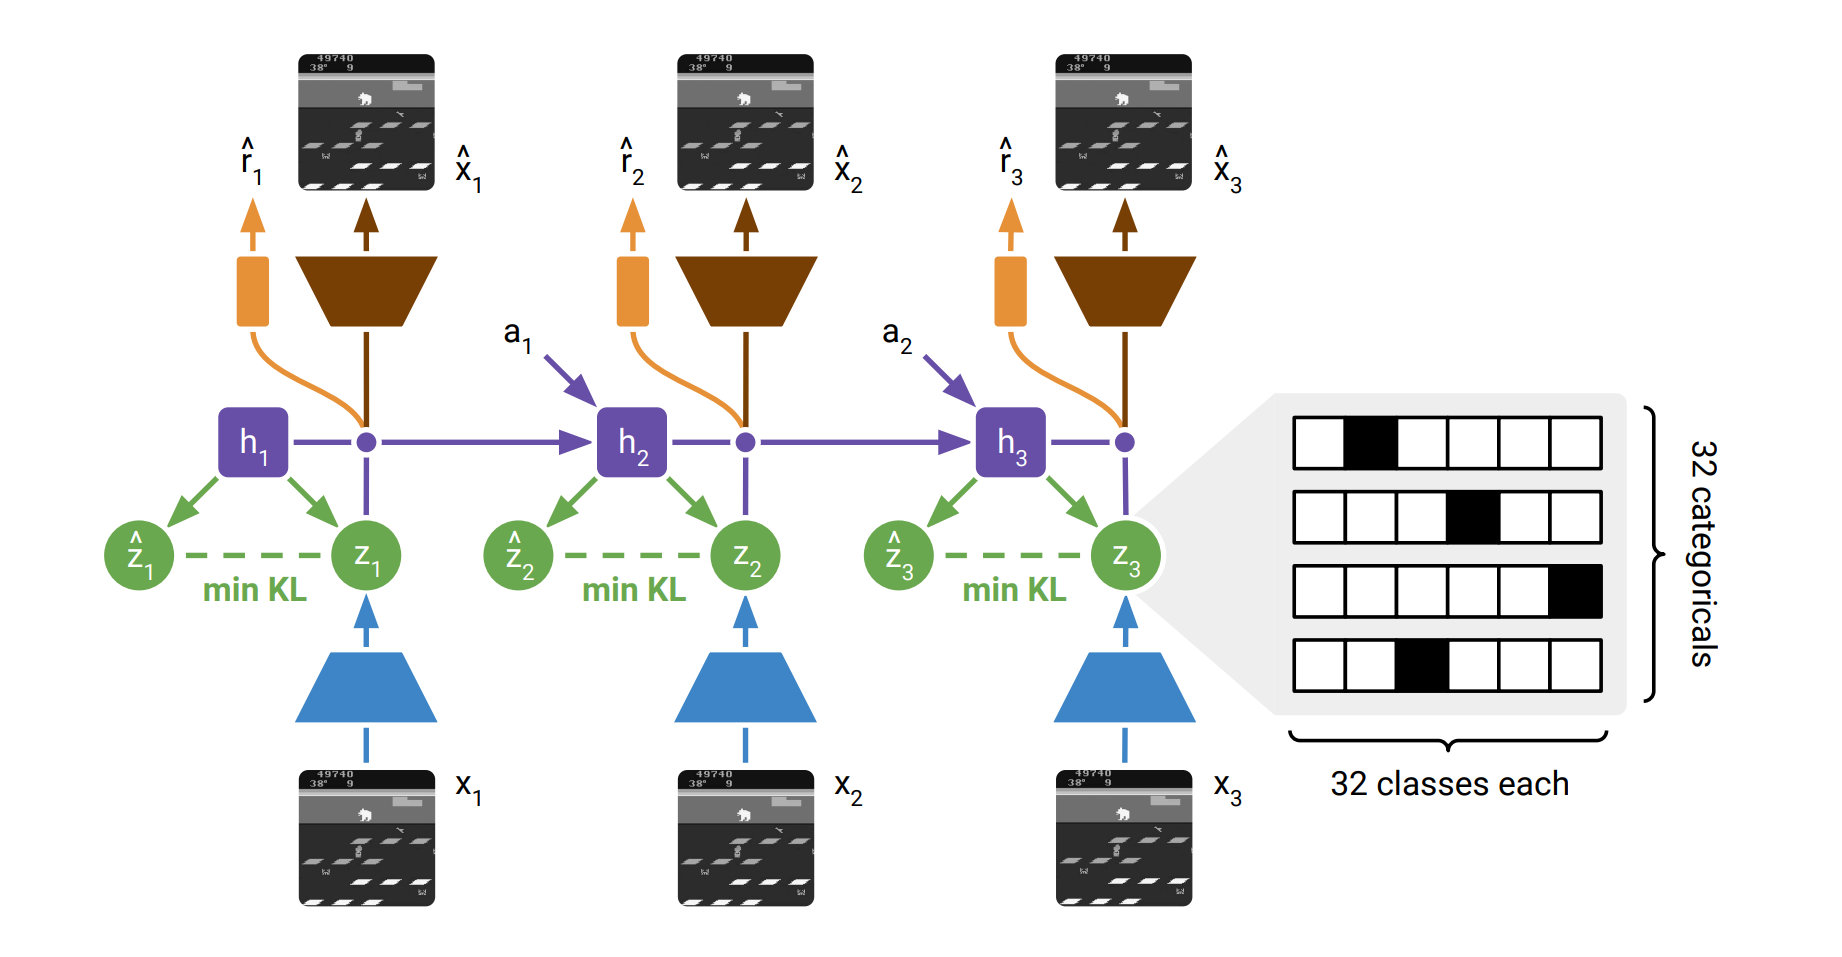
\includegraphics[width=0.9\textwidth]{images/DreamerFlow.png}
	\caption{Overview of the DreamerV2 training pipeline. The world model learns to predict future states and rewards, enabling the actor-critic framework to optimize policies using imagined rollouts.}
	\label{fig:dreamer_flow}
\end{figure}

The $\lambda$-target is defined recursively as:
\begin{equation}
	V^{\lambda}_t = \hat{r}_t + \hat{\gamma}_t \cdot \begin{cases}
		(1 - \lambda)v_\xi(\hat{z}_{t+1}) + \lambda V^{\lambda}_{t+1} & \text{if } t < H \\
		v_\xi(\hat{z}_H)                                              & \text{if } t = H
	\end{cases}
\end{equation}

Here, $\hat{r}_t$ is the predicted reward, $\hat{\gamma}_t$ is the predicted
discount, $v_\xi(\hat{z}_t)$ is the critic value, and $\lambda$ (usually 0.95)
controls how much you care about future rewards. This formula mixes short and
long-term returns.

The actor in DreamerV2 uses a loss that mixes different gradient estimators to
make learning stable. The actor tries to maximize the same $\lambda$-returns as
the critic, using both REINFORCE and backpropagation through the model.

The actor loss is:
\begin{align}
	\mathcal{L}(\psi) = \mathbb{E}\left[\sum_{t=1}^{H-1} \Big[\right. & -\rho \ln p_\psi(\hat{a}_t | \hat{z}_t) \, \text{sg}(V^{\lambda}_t - v_\xi(\hat{z}_t)) \\
	                                                                  & -(1-\rho)V^{\lambda}_t                                                                 \\
	                                                                  & -\eta \mathcal{H}[a_t|\hat{z}_t] \Big]
\end{align}

The loss has three parts:

\textbf{REINFORCE:} Maximizes the log-probability of actions, weighted by the advantage (difference between lambda-return and critic). The stop-gradient (sg) is used to not mess up the critic.

\textbf{Dynamics Backprop:} Backpropagates through the model for more direct gradients.

\textbf{Entropy Regularization:} Encourages exploration by making the action distribution more random. $\eta$ controls how much exploration.

$\rho$ decides how much REINFORCE vs. backprop you use. For Atari, usually $\rho=1$ (just REINFORCE), $\eta=10^{-3}$.

The critic in DreamerV2 estimates the expected return from a latent state. It
is needed for both the lambda-targets and as a baseline for REINFORCE.

The critic is trained with TD learning using the lambda-targets:
\begin{equation}
	\mathcal{L}(\xi) = \mathbb{E}\left[\sum_{t=1}^{H-1} \frac{1}{2} \left(v_\xi(\hat{z}_t) - \text{sg}(V^{\lambda}_t)\right)^2\right]
\end{equation}

Here, $v_\xi(\hat{z}_t)$ is the critic's value, and $\text{sg}(V^{\lambda}_t)$
is the lambda-target with stopped gradients. This helps keep learning stable.

Some tricks are used to make the critic better:

\textbf{Target Network:} Like in DQN, a delayed copy of the critic is used for targets, updated every 100 steps.

\textbf{Trajectory Weighting:} Loss terms are weighted by predicted discounts, so episode ends are handled properly.

\textbf{Latent States:} The critic works on compact latent states, not raw observations, which makes learning faster and more stable.

The critic is usually a small MLP with ELU activations and about 1 million
parameters, outputting a single value for each state. 

Given the advantages of model-based RL and the effectiveness of the Dreamer architecture we now come to the question of how to best
represent the state of the environment.

\section{Object-Centric Reinforcement Learning}
\label{sec:object_centric_rl}

Object-Centric Reinforcement Learning (OCRL) is a collection of methods that do
not make predictions on the raw pixel input but rather try to first create an
abstract representation of the environment which has some semantic
understanding of the objects within it. There are methods that use the pixel
input to create objects from it \cite{locatello2020object,greff2019multi} but
also approaches where the objects states are extracted from RAM
\cite{delfosse2024ocatariobjectcentricatari2600} or given directly by the
environment itself like in JAXAtari

Object-centric model-based RL combine the abstraction of object representations
with state prediction. By using structured object-centric states, agents can
reason about state transitions in a more robust and interpretable way compared
to pixel-based representations. Pixel based representation can thus suffer from
several issues namely:

\begin{itemize}
	\item \textbf{High Dimensionality:} Pixel based inputs are by nature more prone to having more dimensions, making them harder to process and requiring more computational resources.
	\item \textbf{Poor Generalization:} Agents trained on pixel data may struggle to generalize across different environments or object appearances, as they rely heavily on specific visual features and are very prone to slight changes that would not affect human performances but greatly affects the agent \cite{zhang2018dissection,cobbe2019quantifying}.
	\item \textbf{Lack of Semantic Understanding:} Pixel representations do not inherently capture the relationships between objects, limiting the agent's ability to reason about their interactions.
	\item \textbf{Sample Inefficiency:} Learning from high-dimensional pixel data often requires more samples to achieve comparable performance to object-centric approaches \cite{kaiser2019model}.
	\item \textbf{Sensitivity to Noise and Distractors:} Pixel-based methods sometimes focus on irrelevant visual details of the environment which get abstracted away when using object-centric approaches.
\end{itemize}

This object extraction mimics human perception, which naturally segments scenes
into distinct entities and focuses on their interactions
\cite{nanbo2021}.

Therefore object centricity provides several advantages over pixel based
methods.

\textbf{Compositional Understanding:} Object-centric representations naturally excel at treating input features as compositions of distinct entities.
This compositionality allows agents to reason about individual objects and their interactions by for example allowing the agent
to make connections between velocity and the position of a ball to a paddle.

\textbf{Improved Generalization:} By focusing on objects rather than pixel patterns, agents can generalize better across visually different but similar scenarios. For example agents that
understands the concept of a "ball" an an abstract object can use this knowledge in environments where the ball has a different shape or appearance in general \cite{locatello2020object}.

\textbf{Enhanced Interpretability:} Object-centric representations provide naturally a better interpretability than pixel based representations since the agent can reason better that it perceives things as objects rather than "random" pixels.

\textbf{Sample Efficiency:} The structured nature of object-centric representations often leads to more sample-efficient learning. By working with compact, meaningful features rather than high-dimensional
pixel data, agents can learn policies with fewer rollouts. This is possible because the object space is already some kind of latent space which is usually the way things work \cite{hafner2019learning}.

A significant development in this field is the introduction of OCAtari
(Object-Centric Atari) by Delfosse et al.
\cite{delfosse2024ocatariobjectcentricatari2600}. OCAtari extends the
widely-used Arcade Learning Environment (ALE) by providing resource-efficient
extraction of object-centric states for Atari 2600 games. This framework fixes
a gap, where despite growing interest in object-centric approaches, no
standardized benchmark existed for evaluating such methods on the popular Atari
domain.

The OCAtari framework works by two ways of extracting object states. It can
either extract the object states directly from the emulator's RAM or by using
template matching on the rendered frames. The RAM-based extraction is more
efficient and accurate. Directly having those extracted object states allows
for significantly faster training times and also supports researches in making
comparable findings since everyone can use the same object states.

The importance of object-centric approaches in Atari environments is especially
present in light of pixel-based methods in these domains. Delfosse et al.
demonstrated that deep RL agents without interpretable object-centric
representations can learn misaligned policies even in simple games like Pong.
\cite{delfosse2024interpretableconceptbottlenecksalign} This misalignment
problem strengthens the argument for using object-centric understanding rather
than attempting to retrofit interpretability onto pixel-based systems.

Building upon OCAtari, JAXAtari \cite{jaxatari2024} provides a JAX-based
implementation that offers additional performance benefits through just-in-time
compilation and vectorized environments. JAXAtari maintains compatibility with
the object-centric state extraction capabilities of OCAtari while providing
enhanced computational efficiency for large-scale experiments. This framework
is particularly relevant for our work as it enables efficient training of world
models on object-centric representations while maintaining the standardized
benchmarking capabilities essential for reproducible research.

Object-centric representations naturally lend themselves to relational
reasoning, where agents must understand not just individual objects but also
the relationships and interactions between them. This capability is crucial for
complex decision-making in multi-object environments where the optimal policy
depends on understanding how different entities influence each other.

Relational reasoning in reinforcement learning encompasses several key aspects:

\textbf{Spatial Relationships:} Understanding the relative positions of objects and how spatial configurations affect optimal actions. For example, in Pong, the relationship between the paddle position
and ball trajectory determines the appropriate movement strategy.

\textbf{Temporal Relationships:} Tracking how object relationships evolve over time and predicting future interactions. This temporal aspect is particularly important for planning and anticipatory behavior.

\textbf{Causality:} \cite{zambaldi2018deep,battaglia2018relational} Recognizing cause-and-effect relationships between actions and object state changes. This understanding enables more sophisticated planning and can help avoid unintended consequences.

The integration of relational reasoning with model-based approaches offers
significant potential for improving agent performance. By incorporating
relational structure into world models, agents can make more accurate
predictions about future states and plan more effectively. This integration
forms a core component of our proposed approach, where object-centric world
models explicitly encode relational information to enhance both prediction
accuracy and policy learning.

\chapter{Methodology}
\label{chap:methodology}

\section{World Model Architecture}
\label{sec:world_model_arch}

\subsection{LSTM-Based World Model (PongLSTM)}
\label{subsec:ponglstm}
explain LSTM
explain why is might be good for world models in general instead of models that only take the last state into account

\subsection{Alternative Architectures Explored}
\label{subsec:alternative_architectures}
Talk about MLP, Transformer, other RNNs
(TODO) erwähnen dass ich sie ausprobiert habe und warum ich sie nicht genommen habe
(Was ich nicht probiert habe in Future work oder related work)

\subsection{State Normalization and Stability}
\label{subsec:normalization}
why normalization helps in RL in general and why it was used here
(TODO im Background erwähnen dass es Normalisierung in RL gibt und kurz reinschreiben dass ich das gemacht habe)

\section{Actor-Critic Integration}
\label{sec:actor_critic}
Explain how the actor-critic framework is integrated with the object-centric world model.
Discuss any modifications made to the standard actor-critic approach to accommodate the
object-centric representations.

\subsection{DreamerV2-Style Actor-Critic}
\label{subsec:dreamer_ac}
Explain the Dreamer approach and how it differs which is mainly in the latent space

\subsection{Policy Learning in Imagined Rollouts}
\label{subsec:imagined_rollouts}
how the policy is learned in imagined rollouts from the world model

\subsection{Lambda-Return Computation}
\label{subsec:lambda_returns}
provide the formular here and briefly explain it

\section{Training Pipeline}
\label{sec:training_pipeline}
explain when the worldmodel gets retrained and how sampling works

\subsection{World Model Training and experience collection}
\label{subsec:world_model_training}
(TODO Pseudo CODE mit Abbildung)
explain how the initial experience for the world model is collected and how it can be updated during later training stages

\subsection{Policy Optimization}
\label{subsec:policy_optimization}
explain how the policy is optimized and how often

\chapter{Experiments and Results}
\label{chap:experiments}
(QUESTION Soll ich hier Experimente 1,2,3 etc. auflisten und die dann auf die Forschungsfragen mappen
z.B. Experiment 1 10 Schritte unrollst und real vs model vs oc-model bilder -> vielleicht hier einfach
mein OC State Rendern und dann irgendeinen Bild Loss wählen, Dafür muss ich aber ein pixel based world model erstmal haben (einfach ein MLP hinzimmern?))
(Normalen Dreamer zum laufen bringen auch für RQ3 Farbe vom Ball ändern)
(Ablation Studies: Unterschiedliche Architekturen, Unterschiedliche Reward Funktionen)

\section{Experimental Setup}
\label{sec:exp_setup}
* Experimental Design: Baseline, Comparisons, Eval Metrics
* Environment and Setup: Pong Environment Characteristics, Object-Centric State Description
* Hyperparameters and Configuration: Model Architectures, Training Regimes
* Hardware and Implementation Details: Computational Resources, Software Frameworks
* Evaluation Protocol: Training and Testing Procedures, Statistical Analysis

\section{World Model Performance}
\label{sec:world_model_perf}

\subsection{Prediction Accuracy Analysis}
\label{subsec:prediction_accuracy}
Answer here : (RQ1) How does the prediction accuracy of object-centric world models compare to pixel-based world models in terms of state transition prediction and long-term rollout quality in the Pong environment?

\subsection{Long-Term Rollout Quality}
\label{subsec:rollout_quality}
Answer here : (RQ1) How does the prediction accuracy of object-centric world models compare to pixel-based world models in terms of state transition prediction and long-term rollout quality in the Pong environment?

\subsection{Model Stability Assessment}
\label{subsec:stability}
Answer here : (RQ1) How does the prediction accuracy of object-centric world models compare to pixel-based world models in terms of state transition prediction and long-term rollout quality in the Pong environment?

\section{Policy Learning Results}
\label{sec:policy_results}

\subsection{Sample Efficiency Comparison}
\label{subsec:sample_efficiency_comp}
Answer here : (RQ1) To what extent does integrating object-centric representations with model-based RL improve sample efficiency compared to model-free baselines and pixel-based model-based approaches?

\subsection{Final Performance Evaluation}
\label{subsec:final_performance}
Answer here : (RQ1) To what extent does integrating object-centric representations with model-based RL improve sample efficiency compared to model-free baselines and pixel-based model-based approaches?

\subsection{Learning Curve Analysis}
\label{subsec:learning_curves}
Answer here : (RQ1) To what extent does integrating object-centric representations with model-based RL improve sample efficiency compared to model-free baselines and pixel-based model-based approaches?

\section{Ablation Studies}
\label{sec:ablation_studies}

\subsection{Impact of Object-Centric Representations}
\label{subsec:oc_impact}
Answer here : (RQ2) How effectively can the DreamerV2-style actor-critic framework learn optimal policies when trained on imagined rollouts from object-centric world models?

\subsection{Architecture Component Analysis}
\label{subsec:architecture_analysis}
Answer here : (RQ3) What is the impact of different world model architectures (LSTM-based vs. alternatives) on the overall performance of object-centric model-based RL in structured environments?

\subsection{Reward Function Design Effects}
\label{subsec:reward_effects}
Answer here : (RQ3) What is the impact of different world model architectures (LSTM-based vs. alternatives) on the overall performance of object-centric model-based RL in structured environments?

\subsection{Real vs. Model Comparison}
\label{subsec:real_vs_model}
Answer here : (RQ2) How effectively can the DreamerV2-style actor-critic framework learn optimal policies when trained on imagined rollouts from object-centric world models?

\subsection{Policy Behavior Visualization}
\label{subsec:policy_visualization}
Answer here : (RQ2) How effectively can the DreamerV2-style actor-critic framework learn optimal policies when trained on imagined rollouts from object-centric world models?

\chapter{Discussion}
\label{chap:discussion}
* Challenges during training, what decreases model performance

* Analysis of Results
- Strengths of the Proposed Approach
- Limitations and Challenges
- Comparison with Existing Methods

* Technical Insights
- World Model Design Choices
- Training Stability Issues
- Reward Engineering Importance

* Implications for Object-Centric RL
- Benefits of Integration
- Generalization Potential
- Scalability Considerations

* Future Research Directions
- More Complex Environments
- Improved Object Discovery
- Multi-Object Scenarios

\chapter{Conclusion and Future Work}
\label{chap:conclusion}

\begin{itemize}
	\item Summary of Contributions
	\item Key Findings
	\item Limitations and Future Work
	\item Final Remarks
\end{itemize}

\printbibliography[title={References}]

\appendix

\chapter{Implementation Details}
\label{app:implementation}

\section{Code Structure and Organization}
\label{app:code_structure}
Provide an overview of the project's codebase, including the main modules, their purposes, and how they interact.

\section{Hyperparameter Sensitivity Analysis}
\label{app:hyperparameter_analysis}
Discuss the impact of varying key hyperparameters on model performance and training stability.

\section{Additional Experimental Results}
\label{app:additional_results}
Include supplementary experimental results that support the main findings, such as extended comparisons or detailed metrics.

\chapter{Technical Specifications}
\label{app:technical_specs}

\section{Hardware Requirements}
\label{app:hardware_requirements}
List the hardware specifications required to reproduce the experiments, including GPU/CPU details and memory requirements.

\section{Software Dependencies}
\label{app:software_dependencies}
Detail the software libraries, frameworks, and versions used in the implementation.

\section{Reproducibility Guidelines}
\label{app:reproducibility}
Provide step-by-step instructions for reproducing the experiments, including setup, data preparation, and execution.

\chapter{Supplementary Figures and Tables}
Include additional figures and tables that complement the main text, such as
visualizations of training curves or ablation study results.
\label{app:supplementary}

\end{document}